\documentclass[border=6pt]{standalone}
\usepackage{fontspec,unicode-math}
\setmainfont{Noto Serif}
\setmathfont{STIXTwoMath-Regular.otf}
\usepackage{tikz}
\usetikzlibrary{arrows.meta,calc,patterns,decorations.markings,decorations.pathmorphing,decorations.pathreplacing}
\tikzset{lev/.style={line width=1.35pt,line cap=butt},
 fine/.style={line width=.55pt},light/.style={line width=.4pt},
 curve/.style={line width=1.18pt,line cap=round,line join=round},
 ax/.style={line width=.62pt,-{Latex[length=2.15mm,width=1.2mm]}},
 ray/.style={line width=.64pt,-{Latex[length=1.9mm,width=1.0mm]}},
 dim/.style={line width=.52pt,{Latex[length=1.65mm,width=.85mm]}-{Latex[length=1.65mm,width=.85mm]}},
 flow/.style={line width=.60pt,shorten <=1.8pt,shorten >=2.3pt,postaction={decorate},decoration={markings,mark=at position .62 with {\arrow{Latex[length=1.9mm,width=1.0mm]}}}},
 lab/.style={font=\fontsize{13}{16}\selectfont,inner sep=1.5pt},
 small/.style={font=\fontsize{11.2}{13.5}\selectfont,inner sep=1.2pt},
 panel/.style={font=\fontsize{13}{16}\selectfont\itshape,inner sep=1.5pt}}
\pagestyle{empty}
\begin{document}
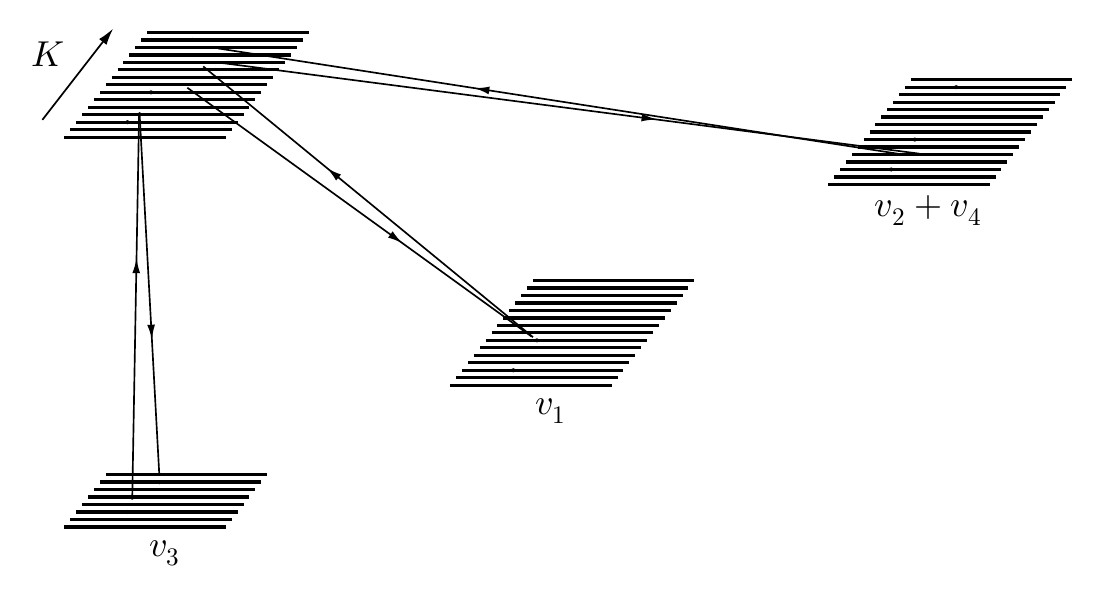
\begin{tikzpicture}[x=1cm,y=1cm,line join=round]
% K-component stacks; slopes and spacings schematic, coupling topology explicit.
\draw[line width=1.18pt] (0.300000,5.250000)--(2.350000,5.250000);
\draw[line width=1.18pt] (0.375000,5.345000)--(2.425000,5.345000);
\draw[line width=1.18pt] (0.450000,5.440000)--(2.500000,5.440000);
\draw[line width=1.18pt] (0.525000,5.535000)--(2.575000,5.535000);
\draw[line width=1.18pt] (0.600000,5.630000)--(2.650000,5.630000);
\draw[line width=1.18pt] (0.675000,5.725000)--(2.725000,5.725000);
\draw[line width=1.18pt] (0.750000,5.820000)--(2.800000,5.820000);
\draw[line width=1.18pt] (0.825000,5.915000)--(2.875000,5.915000);
\draw[line width=1.18pt] (0.900000,6.010000)--(2.950000,6.010000);
\draw[line width=1.18pt] (0.975000,6.105000)--(3.025000,6.105000);
\draw[line width=1.18pt] (1.050000,6.200000)--(3.100000,6.200000);
\draw[line width=1.18pt] (1.125000,6.295000)--(3.175000,6.295000);
\draw[line width=1.18pt] (1.200000,6.390000)--(3.250000,6.390000);
\draw[line width=1.18pt] (1.275000,6.485000)--(3.325000,6.485000);
\draw[line width=1.18pt] (1.350000,6.580000)--(3.400000,6.580000);
\fill (1.100000,5.440000) circle (.026);
\fill (1.400000,5.820000) circle (.026);
\fill (1.925000,6.485000) circle (.026);
\draw[line width=1.18pt] (0.300000,0.300000)--(2.350000,0.300000);
\draw[line width=1.18pt] (0.375000,0.395000)--(2.425000,0.395000);
\draw[line width=1.18pt] (0.450000,0.490000)--(2.500000,0.490000);
\draw[line width=1.18pt] (0.525000,0.585000)--(2.575000,0.585000);
\draw[line width=1.18pt] (0.600000,0.680000)--(2.650000,0.680000);
\draw[line width=1.18pt] (0.675000,0.775000)--(2.725000,0.775000);
\draw[line width=1.18pt] (0.750000,0.870000)--(2.800000,0.870000);
\draw[line width=1.18pt] (0.825000,0.965000)--(2.875000,0.965000);
\fill (1.100000,0.490000) circle (.026);
\fill (1.510000,0.870000) circle (.026);
\fill (1.510000,0.870000) circle (.026);
\node[lab] at (1.580000,-0.030000) {$v_3$};
\draw[line width=1.18pt] (5.200000,2.100000)--(7.250000,2.100000);
\draw[line width=1.18pt] (5.275000,2.195000)--(7.325000,2.195000);
\draw[line width=1.18pt] (5.350000,2.290000)--(7.400000,2.290000);
\draw[line width=1.18pt] (5.425000,2.385000)--(7.475000,2.385000);
\draw[line width=1.18pt] (5.500000,2.480000)--(7.550000,2.480000);
\draw[line width=1.18pt] (5.575000,2.575000)--(7.625000,2.575000);
\draw[line width=1.18pt] (5.650000,2.670000)--(7.700000,2.670000);
\draw[line width=1.18pt] (5.725000,2.765000)--(7.775000,2.765000);
\draw[line width=1.18pt] (5.800000,2.860000)--(7.850000,2.860000);
\draw[line width=1.18pt] (5.875000,2.955000)--(7.925000,2.955000);
\draw[line width=1.18pt] (5.950000,3.050000)--(8.000000,3.050000);
\draw[line width=1.18pt] (6.025000,3.145000)--(8.075000,3.145000);
\draw[line width=1.18pt] (6.100000,3.240000)--(8.150000,3.240000);
\draw[line width=1.18pt] (6.175000,3.335000)--(8.225000,3.335000);
\draw[line width=1.18pt] (6.250000,3.430000)--(8.300000,3.430000);
\fill (6.000000,2.290000) circle (.026);
\fill (6.300000,2.670000) circle (.026);
\fill (6.825000,3.335000) circle (.026);
\node[lab] at (6.480000,1.770000) {$v_1$};
\draw[line width=1.18pt] (10.000000,4.650000)--(12.050000,4.650000);
\draw[line width=1.18pt] (10.075000,4.745000)--(12.125000,4.745000);
\draw[line width=1.18pt] (10.150000,4.840000)--(12.200000,4.840000);
\draw[line width=1.18pt] (10.225000,4.935000)--(12.275000,4.935000);
\draw[line width=1.18pt] (10.300000,5.030000)--(12.350000,5.030000);
\draw[line width=1.18pt] (10.375000,5.125000)--(12.425000,5.125000);
\draw[line width=1.18pt] (10.450000,5.220000)--(12.500000,5.220000);
\draw[line width=1.18pt] (10.525000,5.315000)--(12.575000,5.315000);
\draw[line width=1.18pt] (10.600000,5.410000)--(12.650000,5.410000);
\draw[line width=1.18pt] (10.675000,5.505000)--(12.725000,5.505000);
\draw[line width=1.18pt] (10.750000,5.600000)--(12.800000,5.600000);
\draw[line width=1.18pt] (10.825000,5.695000)--(12.875000,5.695000);
\draw[line width=1.18pt] (10.900000,5.790000)--(12.950000,5.790000);
\draw[line width=1.18pt] (10.975000,5.885000)--(13.025000,5.885000);
\draw[line width=1.18pt] (11.050000,5.980000)--(13.100000,5.980000);
\fill (10.800000,4.840000) circle (.026);
\fill (11.100000,5.220000) circle (.026);
\fill (11.625000,5.885000) circle (.026);
\node[lab] at (11.280000,4.320000) {$v_2+v_4$};
\draw[ax] (0.020000,5.470000)--(0.920000,6.630000);
\node[lab] at (0.080000,6.300000) {$K$};
\coordinate (C0a) at (1.160000,0.585000);\coordinate (C0b) at (1.250000,5.630000);
\draw[flow] (C0a)--(C0b);
\coordinate (C1a) at (1.250000,5.630000);\coordinate (C1b) at (1.510000,0.870000);
\draw[flow] (C1a)--(C1b);
\coordinate (C2a) at (1.810000,5.915000);\coordinate (C2b) at (6.300000,2.670000);
\draw[flow] (C2a)--(C2b);
\coordinate (C3a) at (6.300000,2.670000);\coordinate (C3b) at (2.000000,6.200000);
\draw[flow] (C3a)--(C3b);
\coordinate (C4a) at (2.240000,6.200000);\coordinate (C4b) at (11.240000,5.030000);
\draw[flow] (C4a)--(C4b);
\coordinate (C5a) at (10.950000,5.030000);\coordinate (C5b) at (2.170000,6.390000);
\draw[flow] (C5a)--(C5b);

\end{tikzpicture}
\end{document}
